\newpage
\section{Digitální zpracování signálu}
\subsection{Digitální reprezentace spojitého signálu}
Předpokládejme signál $y(t)$ (např. napětí), který se spojitě mění v čase. Pro uložení a zpracování tohoto signálu na počítači ho měříme v sadě časových okamžiků $t_i$, což nám dává hodnoty signálu $y_i$, a výsledkem je diskrétní reprezentace signálu jako série párů $(t_i, y_i)$. Signál je vzorkován rovnoměrně, pokud $t_i = i\Delta t$, kde $\Delta t$ je \textbf{vzorkovací perioda} a $f_s = 1/\Delta t$ je \textbf{vzorkovací frekvence}.

Jakákoli informace o původním signálu $y(t)$, která se mění v čase rychleji než $\Delta t$, je ztracena. Pokud však $y(t)$ osciluje na frekvenci $f$, nestačí mít $f_s \geq f$. Frekvence signálu $f > f_s/2$ se objeví posunuté na $f - f_s/2$, viz výstup Lst.~\ref{ls:label}. Vzorkovaný signál obsahuje fiktivní frekvence, které v původním signálu nejsou přítomny.

Toto zkreslení se nazývá \textbf{aliasing} a \emph{Nyquistův teorém} říká, že aby se předešlo aliasingu, nejvyšší frekvence obsažená v signálu $f$ nesmí být vyšší než polovina vzorkovací frekvence $f_s/2$, která se nazývá \textbf{Nyquistova frekvence}
\begin{equation}
    \label{eq:nqyust}
    f_N = f_s/2.
\end{equation}

\lstinputlisting[caption=Efekt vzorkovací frekvence, label=ls:label]{../example_code/sampling.py}
\begin{center}
    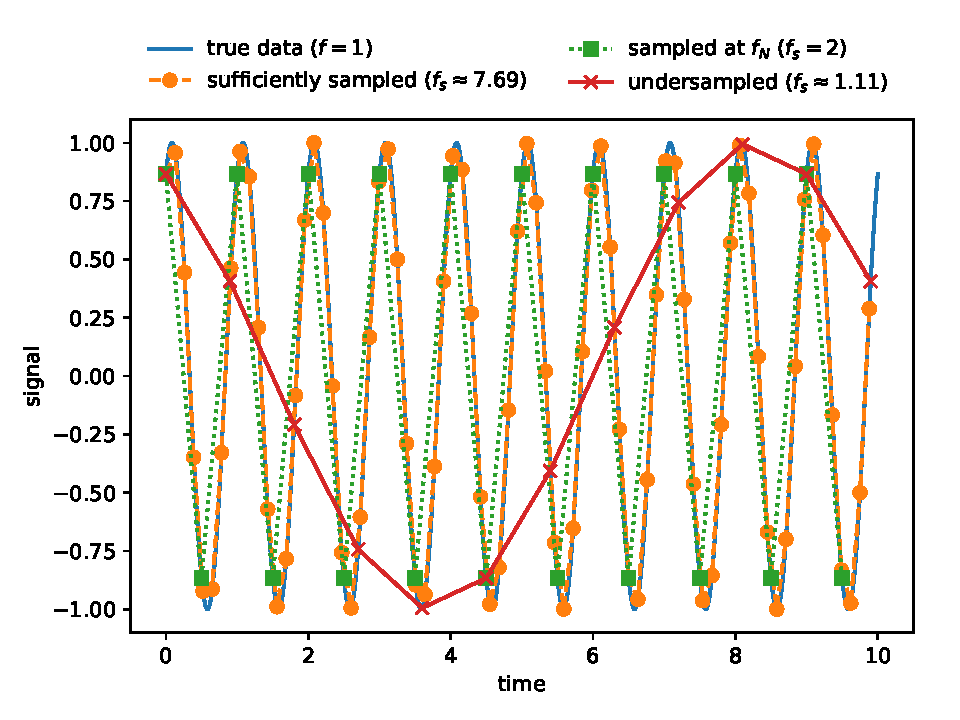
\includegraphics[width=0.75\linewidth]{sampling.pdf}
\end{center}

\subsection{Spektrální analýza}
Jakýkoli periodický signál $y(t)$ (který může být komplexní) s periodou $T$, tj. $y(t + T) = y(t)$, může být reprezentován jako součet sinových a kosinových členů oscilujících na úhlových frekvencích $2\pi n/T$, kde $n$ je celé číslo,
\begin{equation}
    y(t) = \frac{1}{T} \sum_{k=0}^{\infty} A'_k\sin\left(\frac{2\pi k}{T}t\right) + B'_k\cos\left(\frac{2\pi k}{T}t\right),
\end{equation}
což se nazývá \textbf{Fourierova řada}. Ekvivalentně lze Fourierovu řadu vyjádřit pomocí komplexních exponenciál
\begin{equation}
    y(t) = \frac{1}{T} \sum_{k=-\infty}^\infty A_k e^{2\pi ikt/T},
\end{equation}
kde pro reálný signál $y$ jsou kladné a záporné členy komplexně sdružené, $A_k = A_{-k}^*$ (faktor $1/T$ a znaménko uvnitř exponenciální funkce jsou konvenční).

Fourierovy koeficienty $A_k$ lze vypočítat jako
\begin{equation}
    A_k = \int_0^T y(t) e^{-2\pi ikt/T} \mathrm{d}t
\end{equation}

Například, zvažme přímo vypočtenou Fourierovu řadu v Lst.~\ref{lst:fourier-square-pulse}
\lstinputlisting[label=lst:fourier-square-pulse, caption=Fourierova řada obdélníkového pulzu.]{../example_code/fourier_series_square_wave.py}
\begin{center}
    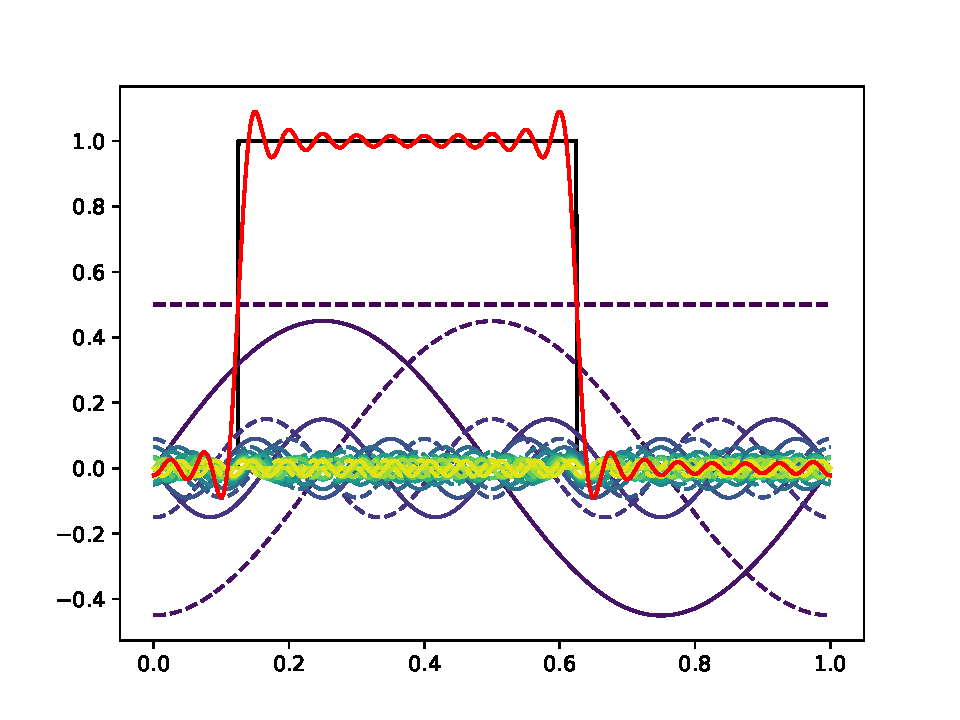
\includegraphics[width=0.5\linewidth]{fourier_series_square_pulse.pdf}
\end{center}

Tyto definice lze rozšířit na aperiodické signály (které si lze představit jako signály s nekonečně dlouhou periodou), což vede k \textbf{Fourierově transformaci}
\begin{equation}
    \tilde y(\omega) = \int_{-\infty}^\infty y(t)e^{-i\omega t} \mathrm{d}t,
\end{equation}
a \textbf{inverzní Fourierově transformaci}
\begin{equation}
    y(t) = \frac{1}{2\pi}\int_{-\infty}^\infty \tilde y (\omega)e^{i\omega t}\mathrm{d}\omega
\end{equation}

Absolutní hodnota Fourierových koeficientů $|A|$ je amplituda oscilace signálu na dané frekvenci a jejich komplexní fáze je fázové posunutí sinových a kosinových členů. Pro Fourierovu transformaci, jelikož se frekvence nyní mění spojitě, má $|\tilde y|$ význam \emph{hustoty} (nazývané spektrální hustota). V analogii s elektrickým výkonem $P = V^2/R$ potřebným k vytvoření napětí $V$ na rezistoru $R$, se $|\tilde y|^2$ nazývá \emph{výkonová spektrální hustota}, tj. $\int_{\omega_0}^{\omega_1} |\tilde y (\omega)|^2\mathrm{d}\omega$ je výkon signálu ve frekvenčním pásmu $(\omega_0, \omega_1)$.

Pro digitální signály mluvíme o \emph{diskrétních} Fourierových transformacích. Pro rovnoměrně vzorkované signály, $t_n = n\Delta t$, jsou tyto v SciPy definovány jako (v podmodulu \ls{scipy.fft})
\begin{equation}
    \tilde y[k] = \sum_{n=0}^{N-1}y[n]e^{-2\pi i kn/N},
\end{equation}
kde $y[n]$ je hodnota signálu $y$ měřená v čase $t_n = n\Delta t$ a $N$ je celkový počet vzorků. Bezrozměrné celočíselné frekvence $k$ probíhají od 0 do $N-1$ -- to znamená, že Fourierova transformace má stejnou délku jako původní signál.

Inverzní diskrétní Fourierova transformace je definována podobně,
\begin{equation}
    y[n] = \frac{1}{N}\sum_{k=0}^{N-1}\tilde y[k]e^{+2\pi i kn/N}.
\end{equation}

Celočíselné frekvenční indexy $k$ reprezentují frekvence $f'_k = k/N$ pro $k=0\dots N/2$ a $f'_k = -k/N$ pro $k=N/2\dots N-1$. Pro získání skutečných frekvencí stačí škálovat $f'_k$ skutečnou vzorkovací frekvencí $1/\Delta t$. Všimněte si, že definice diskrétní Fourierovy transformace a její inverze nezávisí na vzorkovací frekvenci, pouze na tom, že signál je vzorkován rovnoměrně.

Fourierovy transformace jsou implementovány v NumPy a SciPy pomocí algoritmu \textbf{Rychlá Fourierova transformace -- FFT}\footnote{FFT je jedním z nejdůležitějších algoritmů, na kterých závisí celý digitální svět -- např. kódování zvuku a videa a bezdrátová komunikace na něm silně spoléhají.} v podmodulu \ls{scipy.fft}. Fourierova transformace se počítá pomocí \ls{scipy.fft.fft()} a skutečné frekvence lze vypočítat pomocí pomocné funkce \ls{scipy.fft.fftfreq()}. Obě funkce \ls{fft} a \ls{fftfreq} vracejí kladné i záporné frekvence. Pro reálné signály neposkytují záporné frekvence žádné další informace, proto můžeme použít \ls{scipy.fft.rfft()} a \ls{rfftfreq()}, které vracejí pouze kladné frekvence (tj. výsledek má poloviční délku původního signálu). Pokud nás zajímá pouze výkonová spektrální hustota, existuje \ls{scipy.signal.periodogram()}, která také počítá frekvence. Ve výchozím nastavení pro reálné signály vrací \ls{periodogram} pouze kladné frekvence a pro komplexní signály kladné i záporné frekvence. Viz Lst.~\ref{lst:fouriers} pro příklad použití a Lst.~\ref{lst:fft-square-wave} pro verzi programu v Lst.~\ref{lst:fourier-square-pulse}, ale s použitím FFT místo ručního výpočtu koeficientů.

\lstinputlisting[caption=Výpočet Fourierovy transformace a výkonové spektrální hustoty., label=lst:fouriers]{../example_code/fouriers.py}
\begin{center}
    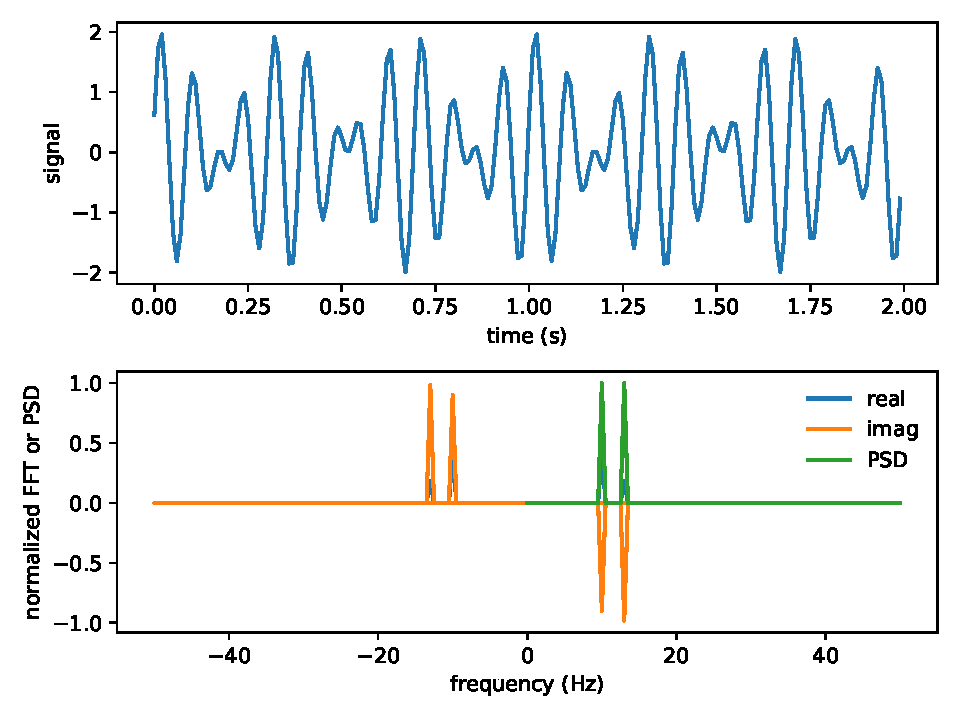
\includegraphics[width=0.5\linewidth]{fouriers.pdf}
\end{center}

\lstinputlisting[label=lst:fft-square-wave, caption=Fourierův koeficient obdélníkové vlny\, vypočtený pomocí FFT]{../example_code/fourier_series_square_wave_fft.py}

Jedna obzvláště důležitá Fourierova transformace je transformace exponenciálně tlumené oscilace, tj.
\begin{equation}
    s(t) = e^{-t/\tau}\sin(2\pi f t),
\end{equation}
což dává komplexní lorentzián, který je odezvou lineárního harmonického oscilátoru, viz sekce~\ref{sec:lho}. Tlumená oscilace je samozřejmě pohyb tlumeného netlumeného lineárního harmonického oscilátoru. Příklad:
\lstinputlisting{../example_code/decaying_exponential.py}
\begin{center}
    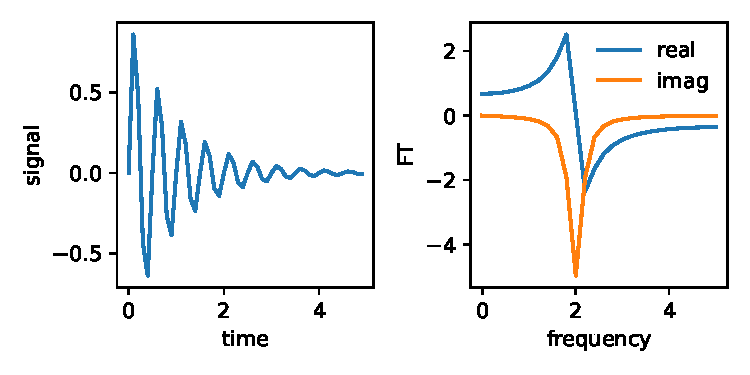
\includegraphics{decaying_exponential.pdf}
\end{center}

\begin{syntax}[Ukládání dat a metadat do binárních souborů numpy.]
    \label{syn:npy}
    Doposud jsme při načítání dat z disku narazili pouze na jednoduché, člověkem čitelné textové soubory. To je velmi omezující způsob ukládání dat: data musí mít formu obdélníkové tabulky, soubory zabírají více místa, než je nutné (např. text \ls{1.234567890} vyžaduje 11 bajtů paměti, ale \ls{float} reprezentující stejné číslo potřebuje pouze 8), a je nepohodlné ukládat metadata.

    Mnoho formátů souborů tyto problémy řeší (např. HDF5 je populární). Zde použijeme řešení, které nevyžaduje žádné další externí knihovny -- ukládání slovníků do komprimovaných binárních souborů \ls{.npy}, např. uložení
\begin{lstlisting}
    raw_data = np.linspace(0, 1, 50)
    my_data = {
        'date of measurement': '20241224',
        'was Mercury in retrograde': False,
        'data': raw_data
    }
    np.save("my_data.npy", my_data)
\end{lstlisting}
    and loading
    a načtení
\begin{lstlisting}
    my_data = np.load("my_data.npy", allow_pickle=True).item()
    print(my_data['date of measurement'])
    print(my_data['data'])
\end{lstlisting}

    \textbf{Pickling} je pythonovský termín pro ukládání téměř jakéhokoli objektu Pythonu na disk jako binární data. Načítání ,,picklovaného'' objektu může být za určitých okolností bezpečnostním rizikem (tj. vyhněte se čtení ,,picklovaných'' dat, která jste stáhli z podivných míst na internetu), proto to musíme explicitně povolit. Funkce \ls{np.load} a \ls{np.save} pracují s poli, proto \ls{np.load()} vrací pole délky 1, kde náš slovník je jediným prvkem. Metoda \ls{array.item()} vrací \ls{array[0]}, pokud má \ls{array} délku 1, jinak vyvolá výjimku \ls{ValueError}. Jejím účelem je sémanticky naznačit, že očekáváme, že pole bude mít pouze jeden prvek, a pokud ne, něco je špatně.
    
    \begin{exercise}
    Načtěte data z adresáře \ls{timeseries_data} a vykreslete časovou závislost přibližné střední teploty během měření. Načtěte soubory pomocí \ls{d = np.load(filename, allow_pickle=True).item()}. Teplota na začátku a na konci měřicího období je \ls{d['Ti']} a \ls{d['Tf']}.
    
    \emph{Nápověda:} Pro získání časového razítka (počet sekund od 00:00 1.1.1970) můžete použít \ls{time.mktime(time.strptime(fn, 'DM_\%Y\%m\%d-\%H\%M\%S.npy'))}, kde \ls{fn} je název souboru.
\end{exercise}
\end{syntax}

\begin{exercise}
    Vykreslete časovou řadu a spektrální hustotu pulzu použitého k buzení rezonance v binárních datových souborech \ls{data/timeseries_data} (viz Ukládání a načítání binárních souborů \ref{syn:npy}) pomocí \ls{scipy.signal.periodogram} a pomocí funkcí (r)FFT z \ls{scipy.fft}. Pulz lze načíst jako \ls{d['pulse']}, počet bodů lze získat jako \ls{d['samples']} (stejné jako \ls{len(d['pulse'])}) a vzorkovací frekvenci jako \ls{d['samples']}. Vykreslete pouze jeden soubor (pulz je pro všechny stejný).
\end{exercise}

\begin{exercise}
    Vykreslete časovou řadu (jako funkci skutečného času) odezvy rezonátoru (\ls{d['timeseries']}) a její frekvenční závislost (reálnou i imaginární složku) pro soubor odpovídající nejnižší teplotě v adresáři \ls{timeseries_data}. Vypočítejte frekvenční odezvu jako poměr Fourierových transformací odezvy rezonátoru a budícího pulzu. Vykreslete pouze frekvence $|f| < 3000$, rezonance je v rozsahu přibližně 2000 - 2400 Hz.
\end{exercise}

\begin{exercise}
    \label{ex:response-heat-map}
    Vykreslete velikost (tj. absolutní hodnotu) odezvy rezonátoru $r$ jako 2D teplotní mapu v závislosti na frekvenci a teplotě (tj. každá řádka v 2D grafu by měla být jedno spektrum odpovídající jedné teplotě).
\end{exercise}

\begin{exercise}
    Jako cvičení~\ref{ex:response-heat-map}, ale zprůměrujte všechna spektra, jejichž teplota je bližší než 50 mK (tato technika vyhlazování se nazývá klouzavý průměr nebo sousední průměrování).
\end{exercise}

\paragraph{Amplitude, power, and decibel}

Při zpracování signálu často mluvíme o útlumu nebo zisku (nebo zesílení) systému, např. kabeláže, zesilovačů nebo atenuátorů. Zisk je definován jako poměr výstupního a vstupního signálu a často se měří v decibelech, definovaných jako
\begin{equation}
    g = 10\log_{10}\frac{s_\mathrm{out}}{s_\mathrm{in}} \mathrm{[dB]}
\end{equation}
nebo pro výkon, tj. $s = V^2$,
\begin{equation}
    g = 20\log_{10}\frac{V_\mathrm{out}}{V_\mathrm{in}}
\end{equation}

Pro ,,absolutní'' veličiny měřené v dB (např. amplituda zvuku je běžná) je měření definováno vzhledem k nějaké dohodnuté referenční hodnotě. Pro zvuk se akustický výkon (tj. druhá mocnina tlaku) měří relativně k 20 \textmu P ve vzduchu. V elektronice, zejména v radiofrekvenčním (RF) inženýrství, je běžnou jednotkou dBm, kde 0 dBm odpovídá 1 mW výkonu, tj. pro zátěž 50 \textohm asi 0.224 V$_\mathrm{RMS}$.

Pro amplitudy odpovídá zdvojnásobení signálu +3 dB a poloviční signál -3 dB a pro výkon je to +6 dB a -6 dB.

\subsection{Filters}

Filtrování je postup, kterým odstraňujeme určité frekvenční rozsahy ze vstupního signálu. Tyto postupy jsou obecné, ale nejjednodušší jsou založeny na analogii s jednoduchými elektronickými RC filtry, viz Obr.~\ref{fig:RC-lowpass}. V závislosti na uspořádání rezistoru a kondenzátoru vytvoříme obvod, který buď zeslabuje nízké, nebo vysoké frekvence.
\begin{figure}
    \centering
    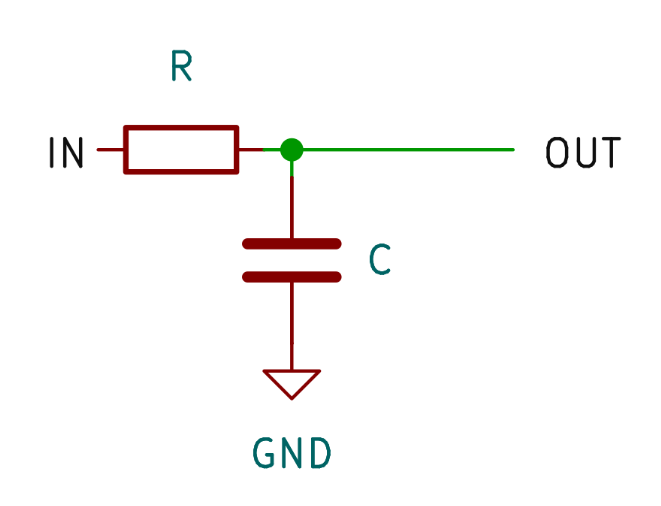
\includegraphics[width=0.49\linewidth]{low-pass-RC.png}%
    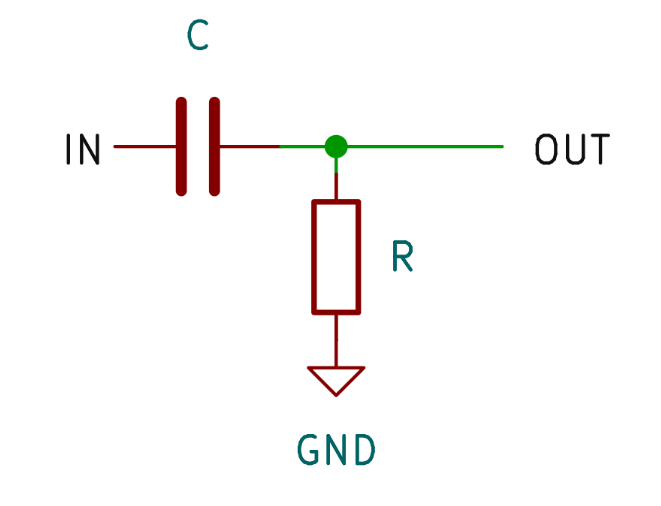
\includegraphics[width=0.49\linewidth]{high-pass-RC.png}%
    \label{fig:RC-lowpass}
    \caption{Dolní propust (vlevo) a horní propust (vpravo) RC filtr.}
\end{figure}

Použitím impedance kondenzátoru $Z_C = (i\omega C)^{-1}$ pro napětí oscilující na úhlové frekvenci $\omega$ dostaneme pro dolní propust
\begin{equation}
    \frac{V_\mathrm{out}}{V_\mathrm{in}} = \frac{1}{1 + i\omega RC},
\end{equation}
a pro horní propust
\begin{equation}
    \frac{V_\mathrm{out}}{V_\mathrm{in}} = \frac{i\omega RC}{1 + i\omega RC}.
\end{equation}
Výše uvedené výrazy se nazývají přenosové funkce filtru. Veličina $RC = \tau$ se nazývá časová konstanta. Mezní frekvence $f_c = 1/(2\pi\tau)$ je frekvence, při které filtr začíná působit. Odezvu filtrů můžeme vykreslit následujícím kódem
\lstinputlisting[firstline=4,lastline=12]{../example_code/RC_filters_response.py}
\begin{center}
    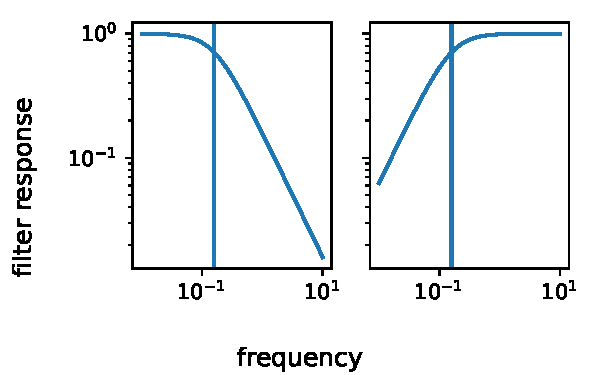
\includegraphics{RC_filters.pdf}
\end{center}
Obrázek ukazuje absolutní hodnotu přenosové funkce pro dolní a horní propust RC filtrů. Svislá čára je mezní frekvence.

Všimněte si, že přenosové funkce jsou funkcemi frekvence a obvody, které reprezentují, jsou lineární, tj. působí na každou frekvenci nezávisle. Proto, pokud je $s(t)$ náš signál a $\hat s(f)$ jeho Fourierova transformace, Fourierova transformace signálu filtrovaného přenosovou funkcí $H(f)$ je jednoduše
\begin{equation}
    \hat s'(f) = H(f)\hat s(f),
\end{equation}
tj. filtry ve frekvenční doméně jednoduše násobí spektrum. V časové doméně $s'(t) = \mathcal{F}^{-1}[H\hat s]$; Fourierova transformace násobení je konvoluce, tj.
\begin{equation}
    s'(t) = (h*s)(t) \equiv \int_{-\infty}^t s(t')h(t - t')\dd t,
\end{equation}
kde $h$ je inverzní Fourierova transformace $H$ a nazývá se konvoluční jádro. Všimněte si, že FFT je často nejrychlejší způsob výpočtu konvoluce, ačkoli ji nemusíme implementovat sami, protože existuje \ls{scipy.signal.convolve(a, b)}, která počítá konvoluci signálů \ls{a} a \ls{b}.

Pro dolní propust RC filtru lze dokázat, že
\begin{equation}
    h(t) = \left\{\begin{matrix}
        e^{-t/\tau} & \mathrm{for}\; t > 0 \\
        0 & \mathrm{for}\; t < 0
    \end{matrix}\right.
\end{equation}
což lze také snadno implementovat pro proudová data, pro která se často nazývá \emph{exponenciální vyhlazování}.

Kromě dolní a horní propusti existují také pásmové propusti a pásmové zádrže. Pásmová propust propouští pouze určité frekvenční pásmo (tj. interval) a pásmová zádrž propouští vše kromě určitého frekvenčního pásma. Pásmovou propust si můžete představit jako horní propust následovanou dolní propustí v sérii a pásmovou zádrž jako dolní a horní propust paralelně s mezními frekvencemi danými propustným nebo zadržovaným pásmem.

Jednoduché RC filtry výše jsou tzv. prvního řádu. Řád filtru udává, jak rychle ořezává signál mimo \emph{propustné pásmo} (tj. interval frekvencí, které filtr propouští). To se často měří v decibelech na oktávu (dB/okt), což udává, o kolik decibelů je signál zeslaben, pokud se jeho frekvence zdvojnásobí, pro dolní propust, nebo zmenší na polovinu pro horní propust, dostatečně daleko od mezní frekvence. Oba RC filtry jsou 6 dB/okt, protože každé zdvojnásobení frekvence odstraní 6 dB přenášeného výkonu.

Rychlejší filtry lze konstruovat jak elektronicky, tak digitálně, ale jak jste viděli v příkladech s krokovou funkcí, ostrý přechod ve spektru vede k oscilacím, které jsou obvykle nežádoucí. Filtry, které jsou maximálně ploché v propustném pásmu, jsou Butterworthovy filtry, pojmenované po Stephenu Butterworthovi, které mají amplitudový zisk
\begin{equation*}
    G_n(\omega) = \frac{1}{\sqrt{1 + \frac{\omega^{2n}}{\omega_c^{2n}}}},
\end{equation*}
kde $\omega_c$ je mezní (úhlová) frekvence. Tyto filtry můžeme zkonstruovat pomocí \ls{scipy.signal.iirfilter} a aplikovat je na náš signál pomocí \ls{scipy.signal.sosfilter}
\lstinputlisting[firstline=7, lastline=25]{../example_code/sig_iirfilter.py}:
\begin{center}
    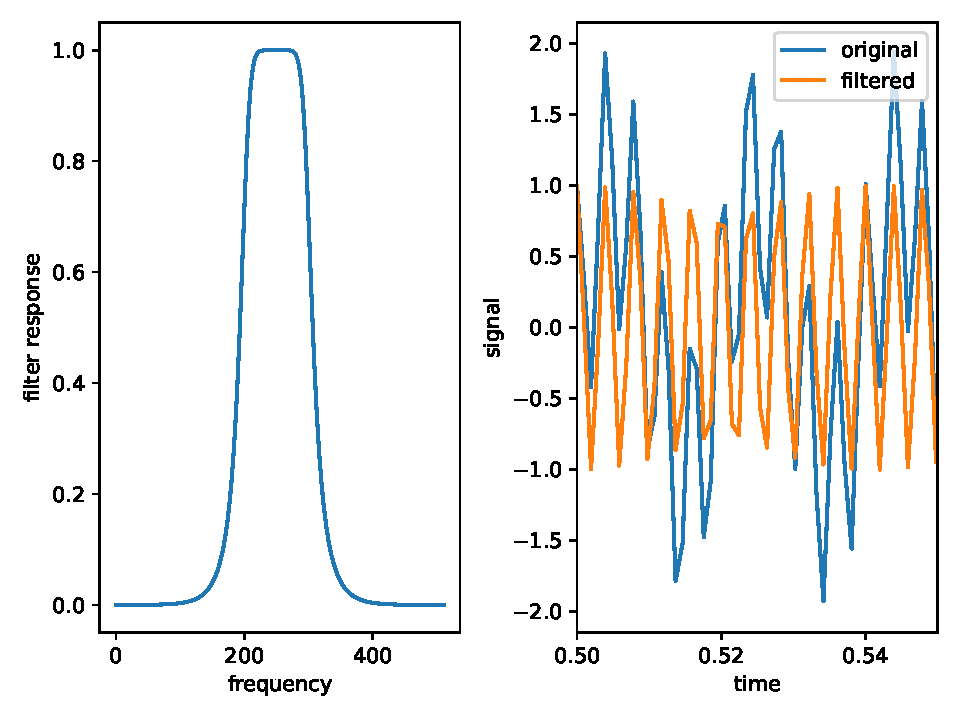
\includegraphics[width=0.5\linewidth]{butter.pdf}
\end{center}

\begin{exercise}
    \label{ex:filter}
    Napište funkci, která bude filtrovat vstupní signál pomocí
    \begin{enumerate}
        \item dolní propusti RC filtru s nastavitelnou mezní frekvencí
        \item horní propusti RC filtru podobně jako v bodě 1.
        \item Butterworthova pásmová propust zkonstruovaná pomocí \ls{scipy.signal.iirfilter()} a aplikovaná pomocí \ls{scipy.signal.lfilter()}
    \end{enumerate}

    Pro 1. a 2. vykreslete přenosovou funkci filtru. Otestujte filtrování na přiloženém \ls{noisy_data.npy} a vykreslete signál v časové i frekvenční doméně před a po filtrování. Pro dolní propust odfiltrujte vše nad 100 Hz. Pro horní propust vše pod 1000 Hz a pro pásmovou propust ponechte pouze rozsah (4310, 4330) Hz.
\end{exercise}

% \subsection{Homodyne and heterodyne detection, signal envelope}
% TODO: mixing, homodyne and heterodyne detection, lock-in amplification

\begin{exercise}
    \label{ex:envelope-direct}
    Demodulujte vyčištěný signál z Cvič.~\ref{ex:filter} (pomocí Butterworthovy pásmové propusti) na nosné frekvenci 4321 Hz (vynásobte $e^{i\omega t}$ a filtrujte dolní propustí) a vykreslete obálku modulující nosnou vlnu.
\end{exercise}

\begin{exercise}
    \label{ex:envelope-hilbert}
    Vypočítejte obálku signálu z Cvič.~\ref{ex:envelope-direct} pomocí Hilbertovy transformace.
\end{exercise}

\subsection{Interpolation and smoothing.}

TODO: \ls{scipy.ndimage.gaussian_filter()}, \ls{scipy.signal.savgol_filter()}, \ls{scipy.interpolate.interp1d()}, \ls{scipy.interpolate.UnivariateSpline()}